% The energy of computing in two places, 1946-2007: in the engineers' specifications and in the economic accounts.
% Figure of the essay "Measured in Kilowatts". Black line work on a transparent ground, Computer Modern,
% 16.2 cm wide (the text column of the site). Adapted from lane 4 of the plate "ict-convergence"
% (Remi-Thesis-GIT-Material, notes/esquisses/2026-10-10_planche-ict-convergence*).
% Build:  pdflatex figure-1-specifications-and-accounts.tex
%         pdftocairo -svg figure-1-specifications-and-accounts.pdf figure-1-specifications-and-accounts.svg
\documentclass[12pt,border=3pt]{standalone}
\usepackage{tikz}
\usetikzlibrary{arrows.meta}
\begin{document}
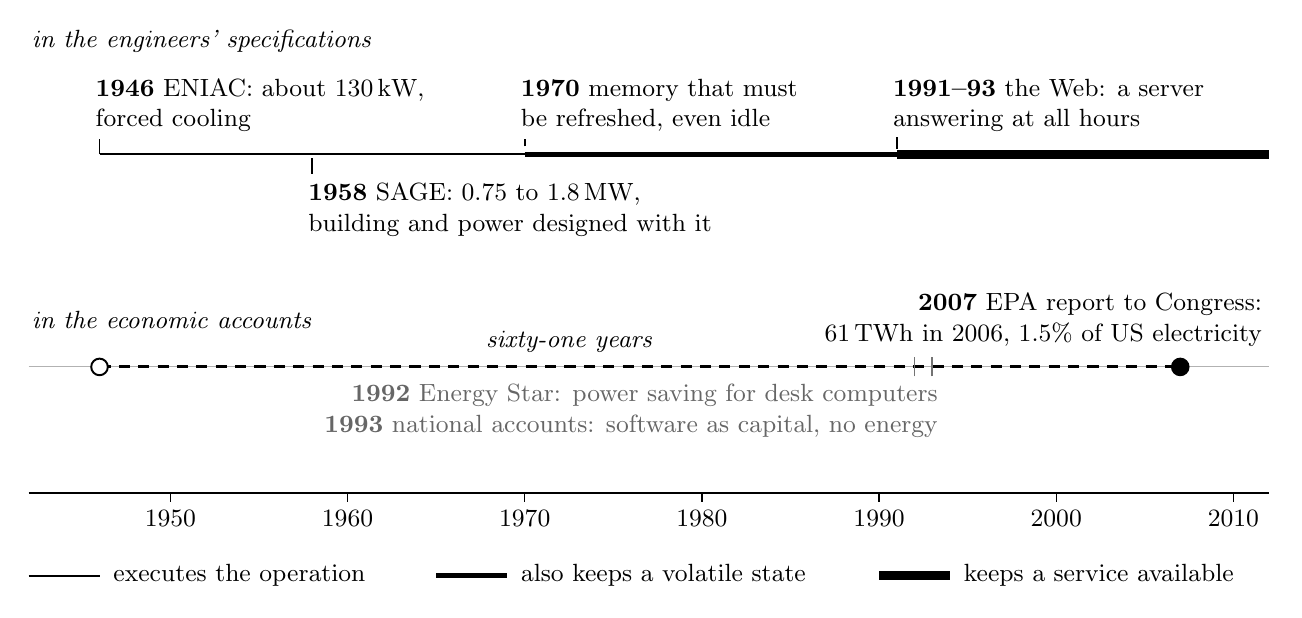
\begin{tikzpicture}[x=0.225cm, y=1cm, font=\small,
  thin/.style={line width=0.7pt},
  medium/.style={line width=1.7pt},
  thick/.style={line width=3.4pt},
  tick/.style={line width=0.6pt},
  lab/.style={inner sep=1pt, align=left},
  labr/.style={inner sep=1pt, align=right},
  lane/.style={inner sep=1pt, font=\small\itshape, anchor=south west},
  grey/.style={text=black!60},
  gap/.style={line width=1.1pt, dash pattern=on 4pt off 3pt}]
\begin{scope}[xshift=-436.95cm]

% ---------------- time axis ----------------
\draw[line width=0.5pt] (1942,0) -- (2012,0);
\foreach \a in {1950,1960,...,2010} {
  \draw[line width=0.5pt] (\a,0) -- (\a,-0.12);
  \node[anchor=north, inner sep=2pt] at (\a,-0.14) {\a};
}

% ---------------- in the specifications ----------------
\node[lane] at (1942,5.55) {in the engineers' specifications};
\draw[thin]   (1946,4.3) -- (1970,4.3);
\draw[medium] (1970,4.3) -- (1991,4.3);
\draw[thick]  (1991,4.3) -- (2012,4.3);

\draw[tick] (1946,4.3) -- (1946,4.5);
\node[lab, anchor=south west] at (1945.6,4.55) {\textbf{1946} ENIAC: about 130\,kW,\\forced cooling};

\draw[tick] (1958,4.25) -- (1958,4.05);
\node[lab, anchor=north west] at (1957.6,3.97) {\textbf{1958} SAGE: 0.75 to 1.8\,MW,\\building and power designed with it};

\draw[tick] (1970,4.4) -- (1970,4.5);
\node[lab, anchor=south west] at (1969.6,4.55) {\textbf{1970} memory that must\\be refreshed, even idle};

\draw[tick] (1991,4.37) -- (1991,4.52);
\node[lab, anchor=south west] at (1990.6,4.55) {\textbf{1991--93} the Web: a server\\answering at all hours};

% ---------------- in the accounts ----------------
\node[lane] at (1942,2.05) {in the economic accounts};
\draw[line width=0.4pt, draw=black!30] (1942,1.6) -- (2012,1.6);
\draw[gap] (1946,1.6) -- (2007,1.6);
\filldraw[fill=white, draw=black, line width=0.7pt] (1946,1.6) circle (3pt);
\filldraw[fill=black, draw=black, line width=0.7pt] (2007,1.6) circle (3pt);
\node[inner sep=1pt, font=\small\itshape, anchor=south] at (1972.5,1.74) {sixty-one years};

\draw[tick, draw=black!55] (1992,1.48) -- (1992,1.72);
\draw[tick, draw=black!55] (1993,1.48) -- (1993,1.72);
\node[labr, grey, anchor=north east] at (1993.5,1.42) {\textbf{1992} Energy Star: power saving for desk computers\\\textbf{1993} national accounts: software as capital, no energy};

\node[labr, anchor=south east] at (2011.8,1.82) {\textbf{2007} EPA report to Congress:\\61\,TWh in 2006, 1.5\% of US electricity};

% ---------------- what the electricity does ----------------
\begin{scope}[yshift=-1.05cm]
  \draw[thin]   (1942,0) -- (1946,0);  \node[lab, anchor=west] at (1946.6,0) {executes the operation};
  \draw[medium] (1965,0) -- (1969,0);  \node[lab, anchor=west] at (1969.6,0) {also keeps a volatile state};
  \draw[thick]  (1990,0) -- (1994,0);  \node[lab, anchor=west] at (1994.6,0) {keeps a service available};
\end{scope}

\end{scope}
\end{tikzpicture}
\end{document}
